\let\negmedspace\undefined
\let\negthickspace\undefined
\documentclass[journal]{IEEEtran}
\usepackage[a4paper, margin=10mm, onecolumn]{geometry}
\usepackage{lmodern} % Ensure lmodern is loaded for pdflatex
\usepackage{tfrupee} % Include tfrupee package

\setlength{\headheight}{1cm} % Set the height of the header box
\setlength{\headsep}{0mm}  % Set the distance between the header box and the top of the text

\usepackage{gvv-book}
\usepackage{gvv}
\usepackage{cite}
\usepackage{amsmath,amssymb,amsfonts,amsthm}
\usepackage{algorithmic}
\usepackage{graphicx}
\usepackage{float}
\usepackage{textcomp}
\usepackage{xcolor}
\usepackage{txfonts}
\usepackage{listings}
\usepackage{enumitem}
\usepackage{mathtools}
\usepackage{gensymb}
\usepackage{comment}
\usepackage[breaklinks=true]{hyperref}
\usepackage{tkz-euclide} 
\usepackage{listings}
% \usepackage{gvv}                                        
\def\inputGnumericTable{}                                 
\usepackage[latin1]{inputenc}                                
\usepackage{color}                                            
\usepackage{array}                                            
\usepackage{longtable}                                       
\usepackage{calc}                                             
\usepackage{multirow}                                         
\usepackage{hhline}                                           
\usepackage{ifthen}                                           
\usepackage{lscape}
\usepackage{tikz}
\usetikzlibrary{patterns}

\begin{document}

\bibliographystyle{IEEEtran}
\vspace{3cm}

\title{1.11.1}
\author{EE25BTECH11064 - Yojit Manral}

\maketitle
% \maketitle
% \newpage
% \bigskip
{\let\newpage\relax\maketitle}
\renewcommand{\thefigure}{\theenumi}
\renewcommand{\thetable}{\theenumi}
\setlength{\intextsep}{10pt} % Space between text and float

\textbf{Question:}\\
Find a vector $\vec{r}$ that is equally inclined to the three axes and whose magnitude is $3\sqrt{3}$ units. \\

\textbf{Solution:}\\
$\rightarrow$ A vector that subtends equal angles to all three axes will have equal components. Let the scaling factor be c. Then,\\

\begin{align}
	\vec{r} &= c\myvec{1\\1\\1} \\
	\implies \norm{\vec{r}} &= \abs{c}\norm{\myvec{1\\1\\1}} \\
	\implies \norm{\vec{r}} &= \abs{c}\sqrt{3} \\
    \text{Given that, } \norm{\vec{r}} &= 3\sqrt{3} \\
	\implies 3\sqrt{3} &= \abs{c}\sqrt{3}\\
	\implies \abs{c} &= 3\\
    \implies \vec{r}&=\myvec{3\\3\\3} \text{ or } \vec{r}=\myvec{-3\\-3\\-3}
\end{align}

\begin{figure}[h!]
   \centering
   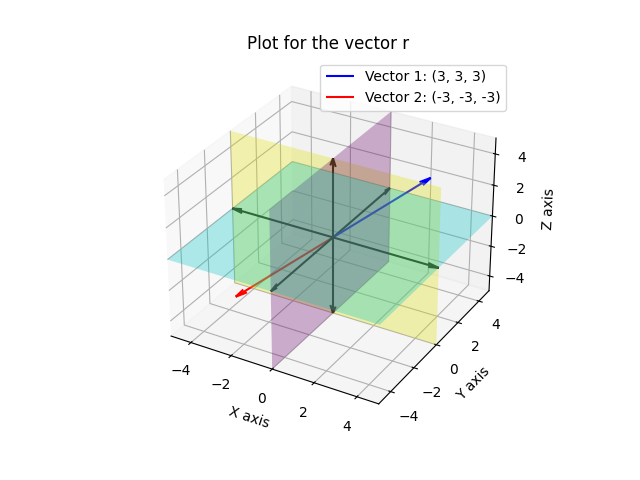
\includegraphics[width=0.8\columnwidth]{figs/01.png}
   \caption{Plot of the vector $\vec{r}$}
   \label{Plot_1}
\end{figure}
\end{document}
